%\documentclass[12pt,letterpaper]{article}

%%%
%% Required packages:
%%
\usepackage{etex}
\usepackage{amsmath}
\usepackage{amssymb}
\usepackage{amstext}
\usepackage{amsthm}
\usepackage{fancyhdr,fancybox}
\usepackage{mathrsfs} % need for \mathscr command
\usepackage{multicol}
\usepackage[normalem]{ulem}
%\usepackage{pictex,pictexplus}
% \usepackage{pictexwd}
\usepackage{rotating}
\usepackage{url}
\usepackage{xfrac}
\usepackage{booktabs}
\usepackage{color,soul}
\usepackage{comment}

\usepackage{hyperref}
\hypersetup{
    colorlinks=true,     % false: boxed links; true: colored links
    linkcolor=blue,      % color of internal links
    citecolor=blue,      % color of links to bibliography
    filecolor=blue,      % color of file links
    urlcolor=blue        % color of external links
}


\usepackage{tikz}
\usetikzlibrary{backgrounds,calc}

%%
%% Common formatting commands
%%
\setlength{\parindent}{0in}
\setlength{\textwidth}{7in}
\setlength{\evensidemargin}{-0.25in}
\setlength{\oddsidemargin}{-0.25in}
\setlength{\parskip}{.5\baselineskip}
\setlength{\topmargin}{-0.5in}
\setlength{\textheight}{9in}

%               Problem and Part
\newcounter{problemnumber}
\newcounter{partnumber}
\newcounter{subpartnumber}
\newcommand{\Problem}{%
  \refstepcounter{problemnumber}%
  \setcounter{partnumber}{0}%
  \setcounter{subpartnumber}{0}%
  \item[\makebox{\hfil\textbf{\theproblemnumber.}\hfil}]%
  }
\newcommand{\InProblem}[2][1.6]{%
  \refstepcounter{problemnumber}%
  \setcounter{partnumber}{0}%
  \setcounter{subpartnumber}{0}%
  \textbf{\theproblemnumber.}\ \ \parbox[t]{#1in}{#2}%
}
\newcommand{\InSmallProblem}[1]{\InProblem[1.05]{#1}}
\newcommand{\NoProblem}[1]{%
  \mbox{\hfil\textbf{#1}\hfil}%
  }
\newcommand{\UnProblem}{%
  \refstepcounter{problemnumber}%
  \setcounter{partnumber}{0}%
  \setcounter{subpartnumber}{0}%
  \mbox{\hfil\textbf{\theproblemnumber.}\hfil}%
  }
\newcommand{\InFlexProblem}[1]{%
  \refstepcounter{problemnumber}%
  \setcounter{partnumber}{0}%
  \setcounter{subpartnumber}{0}%
  \textbf{\theproblemnumber.}\ \ #1%
}
%%  Part:
\newcommand{\Part}{%
  \renewcommand{\thepartnumber}{(\alph{partnumber})}%
  \refstepcounter{partnumber}
  \setcounter{subpartnumber}{0}%
  \item[(\alph{partnumber})]%
}
\newcommand{\InPart}[2][1.75]{%
  \renewcommand{\thepartnumber}{(\alph{partnumber})}%
  \refstepcounter{partnumber}%
  \setcounter{subpartnumber}{0}%
  (\alph{partnumber})\ \ \parbox[t]{#1in}{#2}%
}
\newcommand{\UnPart}{%
  \refstepcounter{partnumber}%
  \renewcommand{\thepartnumber}{(\alph{partnumber})}%
  \setcounter{subpartnumber}{0}%
  (\alph{partnumber})%
}
\newcommand{\InLargePart}[1]{\InPart[3.05]{#1}}
\newcommand{\InFullPart}[1]{\InPart[6.2]{#1}}
\newcommand{\InSmallPart}[1]{\InPart[1.05]{#1}}
%% SubPart:
\newcommand{\SubPart}{%
  \refstepcounter{subpartnumber}%
  \item[(\roman{subpartnumber})]%
  }
\newcommand{\InSubPart}[2][2.25]{%
  \stepcounter{subpartnumber}%
  (\roman{subpartnumber})\ \ \parbox[t]{#1in}{#2}%
}
\newcommand{\InSmallSubPart}[1]{\InSubPart[1.5]{#1}}
\newcommand{\InTinySubPart}[1]{%
  \stepcounter{subpartnumber}%
  (\roman{subpartnumber})\ \ \makebox{#1}%
}
\newcommand{\InMySubPart}[2][2.25]{%
  \stepcounter{subpartnumber}%
  \parbox[t]{#1in}{\makebox[0.3in][l]{(\roman{subpartnumber})}\ \ {#2}}%
}
\newcommand{\TrueFalse}{\textbf{T}\ \ \textbf{F}\ \ }
\newcommand{\TFPart}[1]{% 
  \stepcounter{partnumber}%
  \setcounter{subpartnumber}{0}%
  \item[(\alph{partnumber})] \TrueFalse\parbox[t]{5.5in}{#1}}

\newcommand{\Points}[1]{(#1 points) \ }
\newcommand{\Point}[1]{(#1 point) \ }


%% For Answers:
\newcounter{answernumber}
\newcommand{\Answer}{%
  \refstepcounter{answernumber}%
  \setcounter{partnumber}{0}%
  \setcounter{subpartnumber}{0}%
  \item[\makebox{\hfil\textbf{\theanswernumber.}\hfil}]%
  }


% Setting up the headers for the first page
%\chead{} % will default to what is typed in the file.
\fancyhead[L]{\textsc{Math 22a}}
\fancyhead[R]{\textsc{Fall 2024}}
\fancyfoot[R]{
	\vspace*{\fill}\footnotesize\textcopyright{} \emph{Harvard Math 22a}	
}
\renewcommand{\headrulewidth}{0pt}

%\fancyhead[C]{}
%	\chead{}	
%	\lhead{}
%	\rhead{}
%	\cfoot{}


% Putting copyright on the footer of each page
%\fancypagestyle{secondpage}{
%	\fancyhead[C]{TESTing again} % change this to be blank
%		%\chead{}	
%	\fancyhead[L]{bears} % change this to be blank
%	\fancyhead[R]{dogs} % change this to be blank
%	\fancyfoot[R]{ %keeps the footer the same
%		\vspace*{\fill}\footnotesize\textcopyright{} \emph{Harvard Math 22a}	
%	}
%}
%\renewcommand{\headrulewidth}{0pt}
%\pagestyle{fancy}
\pagestyle{empty}


%\lhead{}
%\rhead{}
%\rfoot{\vspace*{\fill}\footnotesize\textcopyright{} \emph{Harvard Math 22a}}
%\renewcommand{\headrulewidth}{0pt}
%\pagestyle{fancy}




%%
%% Common shortcut commands:
%%
\newcommand{\ds}{\displaystyle}
\newcommand{\sgn}{\operatorname{sgn}}
\renewcommand{\Pr}{\operatorname{P}}
\newcommand{\CPr}[3][{}]{\Pr_{\text{#1}}\left(#2\,|\,#3\right)}

\newcommand{\C}{\mathbb{C}}
\newcommand{\R}{\mathbb{R}}
\newcommand{\Z}{\mathbb{Z}}
\newcommand{\N}{\mathbb{N}}
\newcommand{\Q}{\mathbb{Q}}
\newcommand{\D}{\mathbb{D}}

\newcommand{\rref}{\operatorname{rref}}
\newcommand{\im}{\operatorname{im}}
\newcommand{\rank}{\operatorname{rank}}
\newcommand{\diag}{\operatorname{diag}}
\newcommand{\Span}{\operatorname{span}}
%\renewcommand{\vec}[1]{\mathbf{#1}}
\newcommand{\charpoly}{\mathscr{P}}
\newcommand{\nicefrac}[2]{\sfrac{#1}{#2}} % using xfrac package
\newcommand{\topology}{\mathcal{T}}
\newcommand{\Inn}{\operatorname{Inn}}

\newcommand{\blankbox}[2]{\fbox{\rule{#1}{0in}\rule{0in}{#2}}}

\newenvironment{myindentpar}[1]%
 {\begin{list}{}%
         {\setlength{\leftmargin}{#1}
          \setlength{\rightmargin}{\leftmargin}}%
         \item[]%
 }
 {\end{list}}
\newtheorem{theorem}{Theorem}
\newtheorem*{NStheorem}{Theorem}
\newtheorem{cor}[theorem]{Corollary}
\newtheorem*{claim}{Claim}
\newtheorem{defn}{Definition}

\newenvironment{amatrix}[1]{%
  \left(\begin{array}{@{}*{#1}{c}|c@{}}
}{%
  \end{array}\right)
}

%--------grstep
% For denoting a Gauss' reduction step.
% Use as: \grstep{\rho_1+\rho_3} or \grstep[2\rho_5 \\ 3\rho_6]{\rho_1+\rho_3}
\newcommand{\grstep}[2][\relax]{%
   \ensuremath{\mathrel{
       {\mathop{\longrightarrow}\limits^{#2\mathstrut}_{
                                     \begin{subarray}{l} #1 \end{subarray}}}}}}
\newcommand{\swap}{\leftrightarrow}



\section{{Set Theory,  \framebox\S 1, 8} and Proof Methods, \framebox\S 4,  5,  6}
\chead{\Large\textbf{Set Theory,  \fbox\S 1, 8}}

%\begin{document}
\thispagestyle{fancy}

\begin{enumerate}
  \Problem Let $A = \{12 n \;\big{|}\; n \in \Z\}$, and let $B =
  \{k\in \Z\;\big{|}\; k\ \text{is even}\}$, and let $C= \{3j
  \;\big{|}\; j \in \Z\}$.  Show that $A \subseteq B\cap C$.  That is,
  show that if $x\in A$, then $x\in B$ \emph{and}\ $x\in C$.
  \vfill

\end{enumerate}

\newpage

Let's start with some notation and
visual intuition.  Generally speaking we'll be drawing an example as
below, with $A$ and $B$ as subsets of a larger ``universe'' $S$.
\begin{center}
  \begin{tikzpicture}[x=7.5mm,y=7.5mm,>=latex]
    \draw[ultra thick, black, rounded corners=4mm] (0,0) rectangle (5,3);
    \draw[thick, black] (1.5,1.5) circle (0.75);
    \draw[thick, black, rounded corners=2mm] (2.0,0.65) rectangle (4.0,2.35);
    \node at (0.7,2.3) {\small$A$};
    \node at (3.65,2.65) {\small$B$};
    \node at (5.35,2.55) {\small$S$};
  \end{tikzpicture}
\end{center}
\begin{center}
  \begin{tabular}{cccp{2.2in}}
    \makebox[1in][c]{\large\textbf{Operation}}
    & \makebox[1in][c]{\large\textbf{Expression}}
    & {\large\textbf{Picture}}
    & {\large\textbf{Description/Definition}} \\ \toprule 
    \makebox[1in][c]{Union} & \makebox[1in][c]{$A \cup B$}
    & 
      \begin{tikzpicture}[x=7.5mm,y=7.5mm,>=latex,baseline=12.5mm]
        \draw[ultra thick, black, rounded corners=4mm] (0,0) rectangle (5,3);
        \fill[gray!20] (1.5,1.5) circle (0.75);
        \fill[gray!20, rounded corners=2mm] (2.0,0.65) rectangle (4.0,2.35);
        \draw[thick, black] (1.5,1.5) circle (0.75);
        \draw[thick, black, rounded corners=2mm] (2.0,0.65) rectangle (4.0,2.35);
        \node at (0.7,2.3) {\small$A$};
        \node at (3.65,2.65) {\small$B$};
        \node at (5.35,2.55) {\small$S$};
      \end{tikzpicture}
    &$x\in A\cup B$ iff $x\in A$ or $x\in B$.
    \\[1.5cm]
    Intersection & $A \cap B$
    & 
      \begin{tikzpicture}[x=7.5mm,y=7.5mm,>=latex,baseline=12.5mm]
        \draw[ultra thick, black, rounded corners=4mm] (0,0) rectangle (5,3);
        \begin{scope}
          \clip[rounded corners=2mm] (2.0,0.65) rectangle (4.0,2.35);
          \fill[gray!20] (1.5,1.5) circle (0.75);
        \end{scope}
        \draw[thick, black] (1.5,1.5) circle (0.75);
        \draw[thick, black, rounded corners=2mm] (2.0,0.65) rectangle (4.0,2.35);
        \node at (0.7,2.3) {\small$A$};
        \node at (3.65,2.65) {\small$B$};
        \node at (5.35,2.55) {\small$S$};
      \end{tikzpicture}
    &$x\in A\cap B$ iff $x\in A$ and $x\in B$.
    \\[1.5cm]
    Set difference & $A \smallsetminus B$
    & 
      \begin{tikzpicture}[x=7.5mm,y=7.5mm,>=latex,baseline=12.5mm]
        \draw[ultra thick, black, rounded corners=4mm] (0,0) rectangle (5,3);
        \fill[gray!20] (1.5,1.5) circle (0.75);
        \fill[white,rounded corners=2mm] (2.0,0.65) rectangle (4.0,2.35);
        \draw[thick, black] (1.5,1.5) circle (0.75);
        \draw[thick, black, rounded corners=2mm] (2.0,0.65) rectangle (4.0,2.35);
        \node at (0.7,2.3) {\small$A$};
        \node at (3.65,2.65) {\small$B$};
        \node at (5.35,2.55) {\small$S$};
      \end{tikzpicture}
    &$x\in A\smallsetminus B$ iff $x\in A$ and $x\not\in B$.
    \\[1.5cm]
    Complement & $A'$ (or $A^c$ or $\overline{A}$)
    & 
      \begin{tikzpicture}[x=7.5mm,y=7.5mm,>=latex,baseline=12.5mm]
        \fill[gray!20, rounded corners=4mm] (0,0) rectangle (5,3);
        \draw[ultra thick, black, rounded corners=4mm] (0,0) rectangle (5,3);
        \fill[white] (1.5,1.5) circle (0.75);
        \draw[thick, black] (1.5,1.5) circle (0.75);
        \draw[thick, black, rounded corners=2mm] (2.0,0.65) rectangle (4.0,2.35);
        \node at (0.7,2.3) {\small$A$};
        \node at (3.65,2.65) {\small$B$};
        \node at (5.35,2.55) {\small$S$};
      \end{tikzpicture}
    &$x\in A'$ iff $x\not\in A$.
    \\[1.5cm]
    Subset & $A\subseteq B$ (or $B\supseteq A$)
    & 
      \begin{tikzpicture}[x=7.5mm,y=7.5mm,>=latex,baseline=12.5mm]
        % \fill[gray!20, rounded corners=4mm] (0,0) rectangle (5,3);
        \draw[ultra thick, black, rounded corners=4mm] (0,0) rectangle (5,3);
        \fill[gray!20] (2.5,1.5) circle (0.65);
        \draw[thick, black] (2.5,1.5) circle (0.65);
        \draw[thick, black, rounded corners=2mm] (1.0,0.65) rectangle (4.0,2.35);
        \node at (1.65,1.9) {\small$A$};
        \node at (3.65,2.65) {\small$B$};
        \node at (5.35,2.55) {\small$S$};
      \end{tikzpicture}
    &$x\in A \implies x\in B$.
  \end{tabular}
\end{center}

\newpage

For each of the following, determine whether the statement is true for
all sets $A$, $B$ and $C$.  If an equality fails, determine whether
one or the other of the possible inclusions holds. Prove your
assertions.


\begin{enumerate}
  \Problem $(A\cap B) \cup (A\smallsetminus B) = A$
  \vfill

  \Problem $A\cup (B\smallsetminus C) = (A\cup B) \smallsetminus (A\cup C)$
  \vfill
  
 % \Problem $A \times (B\smallsetminus C) = (A\times B) \smallsetminus (A\times C)$
%  \vfill
  
   \Problem\label{prob:1}%
  Suppose $A = \{ k\in\Z\;|\;3|k\}$ and $B=\{2k\;|\;k\in\Z\}$ are
  subsets of $\Z$.  Describe (a) $\left(A \cup B \right)'$ and (b)
  $\left(A \cap B \right)'$.  
  \vfill
\end{enumerate}

%
%\end{document}

\begin{comment}

\newpage
\chead{\Large\textbf{The Joy of Sets -- Solutions and Comments}}
\lhead{}
\rhead{}
\thispagestyle{fancy}



Now, on to the solutions!

\begin{enumerate}
  \Answer If $x\in A$, then $x=12n$ for some integer $n$.  Thus
  $x=2(6n)$ (so $x\in B$) and $x=3(4n)$ (so $x\in C$), and therefore
  $x\in B\cap C$.  That is, $A \subseteq B\cap C$.

  \Answer\label{ans:2}%
  This seems to be true from a quick sketch (see Figure~\ref{fig:ans2}).
  \begin{figure}[htbp]
    \centering
    % $(A \cap B) \cup (A\smallsetminus B) = $
    \begin{tikzpicture}[x=7.5mm,y=7.5mm,>=latex,baseline=10mm]
      \draw[ultra thick, black, rounded corners=4mm] (0,0) rectangle (5,3);
      \begin{scope}
        \clip[rounded corners=2mm] (2.0,0.65) rectangle (4.0,2.35);
        \fill[gray!20] (1.5,1.5) circle (0.75);
      \end{scope}
      \draw[thick, black] (1.5,1.5) circle (0.75);
      \draw[thick, black, rounded corners=2mm] (2.0,0.65) rectangle (4.0,2.35);
      \node at (0.7,2.3) {\small$A$};
      \node at (3.65,2.65) {\small$B$};
      % \node at (5.35,2.55) {\small$S$};
      \node at (2.5,-0.5) {$A\cap B$};
    \end{tikzpicture}
    $\displaystyle\cup$
    \begin{tikzpicture}[x=7.5mm,y=7.5mm,>=latex,baseline=10mm]
      \draw[ultra thick, black, rounded corners=4mm] (0,0) rectangle (5,3);
      \fill[gray!20] (1.5,1.5) circle (0.75);
      \fill[white,rounded corners=2mm] (2.0,0.65) rectangle (4.0,2.35);
      \draw[thick, black] (1.5,1.5) circle (0.75);
      \draw[thick, black, rounded corners=2mm] (2.0,0.65) rectangle (4.0,2.35);
      \node at (0.7,2.3) {\small$A$};
      \node at (3.65,2.65) {\small$B$};
      % \node at (5.35,2.55) {\small$S$};
      \node at (2.5,-0.5) {$A\smallsetminus B$};
    \end{tikzpicture}
    $=$
    \begin{tikzpicture}[x=7.5mm,y=7.5mm,>=latex,baseline=10mm]
      \draw[ultra thick, black, rounded corners=4mm] (0,0) rectangle (5,3);
      \fill[gray!20] (1.5,1.5) circle (0.75);
      \draw[thick, black] (1.5,1.5) circle (0.75);
      \draw[thick, black, rounded corners=2mm] (2.0,0.65) rectangle (4.0,2.35);
      \node at (0.7,2.3) {\small$A$};
      \node at (3.65,2.65) {\small$B$};
      % \node at (5.35,2.55) {\small$S$};
      \node at (2.5,-0.5) {$A$};
    \end{tikzpicture}
    % $ = A$.
    \caption{A quick sketch for the answer to Problem~\ref{ans:2}}
    \label{fig:ans2}
  \end{figure}
  As usual, to prove two sets are equal, we prove each is a subset of
  the other.  That is, to prove $S=T$, we prove that $S\subseteq T$ and
  $S\supseteq T$.  We'll do this in parts:
  \begin{enumerate}
    \Part $(A\cap B) \cup (A\smallsetminus B) \subseteq A$

    If $x \in (A\cap B) \cup (A\smallsetminus B)$, then either $x\in A
    \cap B$ (in which case $x\in A$) or $x\in A\smallsetminus B$ (and
    again $x\in A$).  Thus $x\in A$.
    \medskip

    \Part $A \subseteq (A\cap B) \cup (A\smallsetminus B)$

    Suppose $x\in A$.  If $x\in B$, then $x\in A\cap B$.  If $x\not\in
    B$, then $x\in A\smallsetminus B$.  Combining these, we see that
    $x\in (A\cap B) \cup (A\smallsetminus B)$.

  \end{enumerate}

  \Answer This is \emph{not true}, since any element of $A$ is
  included in the set on the left but is not included in the set on
  the right (it gets ``subtracted away'' when we remove $A\cup C$ from
  $A\cup B$).  Only one inclusion holds:
  \medskip

  \textbf{Claim:}\ $(A\cup B) \smallsetminus (A\cup C) \subseteq A\cup (B\smallsetminus C)$

  \begin{proof}
    Let $x\in (A\cup B) \smallsetminus (A\cup C)$.  Then $x\in A\cup
    B$ and $x\not\in A\cup C$.  That is, $x$ is an element of either
    $A$ or $B$ \textbf{AND}\ $x$ is an element of neither $A$ nor $C$.
    That is, $x\not\in A$, $x\in B$ and $x\not\in C$.  Thus $x\in
    B\smallsetminus C$, so $x\in A \cup (B\smallsetminus C)$.
  \end{proof}


%%  \Answer Again we prove this in two steps, showing that each set is a
%  subset of the other:
%  \begin{enumerate}
%    \Part $A \times (B\smallsetminus C) \subseteq (A\times B) \smallsetminus (A\times C)$
%
%    If $(x,y) \in A \times (B\smallsetminus C)$, then $x\in A$, $y\in
%    B$ and $y\not\in C$.  Thus $(x,y) \in A\times B$ and $(x,y)\not\in
%    A\times C$, so $(x,y) \in (A\times B) \smallsetminus (A\times C)$.
%    \medskip
%
%    \Part $(A\times B) \smallsetminus (A\times C) \subseteq A \times (B\smallsetminus C)$
%
%    Now suppose $(x,y) \in (A\times B) \smallsetminus (A\times C)$.
%    This means $(x,y) \in A\times B$, so $x\in A$ and $y\in B$.  It
%    also means $(x,y)\not\in A\times C$.  But we've seen $x\in A$, so
%    the only way for $(x,y)$ to fail to be an element of $A\times C$
%    is for $y$ to not be in $C$: $y\not\in C$.  Thus $x\in A$ and
%    $y\in B\smallsetminus C$, so $(x,y) \in A \times (B\smallsetminus C)$.

%  \end{enumerate}
  
  \Answer
  Here $A\cup B$ can be described as all integers that are multiples
  of $2$ or $3$.  The complement is therefore all integers that are
  \emph{not}\ multiples of $2$ or $3$.  Written out explicitly, we get
  \begin{equation*}
    \left(A \cup B \right)'
    = \left\{ \pm1\,,\,\pm5\,,\,\pm7\,,\,\pm11\,,\,\pm13\,,\,\pm17\,,\,\pm19\,,\,\pm23\,,\,\pm25\,,\,\pm29\,,\,\pm31\,,\,\pm35\,,\,\ldots\right\}.
  \end{equation*}
  The intersection $A\cap B$ is the set of all integers that are
  multiples of \emph{both}\ $2$ and $3$ -- that is, it is the set of
  integers that are multiples of $6$.  The complement is thus all
  integers that are not divisible by $6$:
  \begin{equation*}
    \left(A \cap B \right)'
    = \left\{ \pm1\,,\,\pm2\,,\,\pm3\,,\,\pm4\,,\,\pm5\,,\,\pm7\,,\,\pm8\,,\,\pm9\,,\,\pm10\,,\,\pm11\,,\,\pm13\,,\,\ldots\right\}.
  \end{equation*}

Part of the point of Problem~\ref{prob:1}\ is to introduce the
set-theoretic versions of
\href{https://en.wikipedia.org/wiki/De_Morgan\%27s_laws#Set_theory_and_Boolean_algebra}{De
  Morgan's Laws:}
\begin{equation*}
    \left(A \cup B \right)'
    = A' \cap B'
    \qquad\text{and}\qquad
    \left(A \cap B \right)'
    = A' \cup B'.
\end{equation*}
Here are the pictures to illustrate what's going on.  Here's our
entire set $S$, with the circular set $A$ and the rectangular set $B$:
\begin{center}
  \begin{tikzpicture}[x=15mm,y=15mm,>=latex]
    \draw[ultra thick, black, rounded corners=4mm] (0,0) rectangle (5,3);
    \draw[thick, black] (1.5,1.5) circle (0.75);
    \draw[thick, black, rounded corners=2mm] (2.0,0.65) rectangle (4.0,2.35);
    \node at (0.8,2.2) {$A$};
    \node at (2.45,2.55) {$B$};
    \node at (5.25,2.7) {$S$};
  \end{tikzpicture}
\end{center}
Then here are $A\cup B$ (left) and $A'\cap B'$ (right), showing that
$(A\cup B)' = A'\cap B'$:
\begin{center}
  \begin{tabular}{ccc}
    \begin{tikzpicture}[x=15mm,y=15mm,>=latex]
      \draw[ultra thick, black, rounded corners=4mm] (0,0) rectangle (5,3);
      \draw[thick, black, fill=gray,fill opacity=0.2] (1.5,1.5) circle (0.75);
      \draw[thick, black, rounded corners=2mm, fill=gray,fill opacity=0.2] (2.0,0.65) rectangle (4.0,2.35);
      \node at (0.8,2.2) {$A$};
      \node at (2.45,2.55) {$B$};
      \node at (5.25,2.7) {$S$};
    \end{tikzpicture}
    & \hspace*{0.25in} & 
    \begin{tikzpicture}[x=15mm,y=15mm,>=latex]
      \draw[ultra thick, black, rounded corners=4mm,fill=gray,fill opacity=0.2] (0,0) rectangle (5,3);
      \draw[thick, black, rounded corners=2mm,fill=white] (2.0,0.65) rectangle (4.0,2.35);
      \draw[thick, black,fill=white] (1.5,1.5) circle (0.75);
      \draw[thick, black, rounded corners=2mm] (2.0,0.65) rectangle (4.0,2.35);
      \node at (0.8,2.2) {$A$};
      \node at (2.45,2.55) {$B$};
      \node at (5.25,2.7) {$S$};
    \end{tikzpicture}
    \\
    $A\cup B$ (shaded), so $(A\cup B)'$ is in white
    && 
    $A'\cap B'$ is shaded
  \end{tabular}
\end{center}
The other law is proved similarly; you can draw the diagram yourself.
\end{enumerate}

%\end{document}
\end{comment}

%%% Local Variables: 
%%% mode: latex
%%% TeX-master: t
%%% End: 
